
\chapter{Abstract Variational Problems and Examples}\label{chap2}

IN\pageoriginale SECTION 1 OF this chapter, we give a variational
formulation of the Dirichlet problem. In section 2 we prove the
existence and uniqueness results for the abstract variational
problem. In the remaining sections, we deal with the Neumann problem,
Elasticity problem, Stokes problem and Mixed problem and their
variational formulations.

\section{Dirichlet Problem}\label{chap2:ssec2.1} 
The Dirichlet problem is to find $u$ such that 
\begin{align}\label{chap2:eq2.1}
-\Delta u &= f \quad \text{in} \quad \Omega \\
u &= 0 \quad \text{on} \quad \Gamma \label{chap2:eq2.2}
\end{align}
where $\Omega \subset \mathbb{R}^n$ is a bounded open set with smooth
boundary $\Gamma$ and $f$ is a given function. 

Multiplying equation \eqref{chap2:eq2.1} by a smooth function $v$
which vanishes on $\Gamma$ and integrating, we obtain 
\begin{equation}\label{chap2:eq2.3}
\int\limits_\Omega -\Delta u.v \,dx = \int\limits_\Omega f.v \,dx
\end{equation}

Formally, using integration by parts and the fact that $v=0$ on
$\Gamma$, we see that 
\begin{equation}\label{chap2:eq2.4}
\int\limits_\Omega\nabla v.\nabla u \,dx=\int\limits_\Gamma\frac{\partial
  u}{\partial n}v \, d\Gamma - \int\limits_\Omega\Delta u \; v \,dx=
\int\limits_\Omega -\Delta u.v \,dx 
\end{equation}
Equations \eqref{chap2:eq2.3} and \eqref{chap2:eq2.4} give 
$$
\int\limits_\Omega \nabla u.v \,dx=\int\limits_\Omega f\; v\,dx.
$$
Now, setting 
$$
a(u, v)=\int\limits_\Omega \nabla u.\nabla v \,dx
$$\pageoriginale
and 
$$
L(v)=\int\limits_\Omega fv \,dx,
$$
problem \eqref{chap2:eq2.1} can be formulated thus:

\noindent Find $u \varepsilon V$ such that 
\begin{equation}\label{chap2:eq2.5}
a(u, v)=L(v) \quad \text{for all }  v \varepsilon V,
\end{equation}
where $V$ has to be chosen suitably.

Since $a(\cdotp,\cdotp)$ is symmetric, \eqref{chap2:eq2.5} is Euler's condition for
the minimization problem 
\begin{equation}\label{chap2:eq2.6}
J(u)=\inf\limits_{v\varepsilon V} J(v),
\end{equation}
where
$$
J(v)=1/2 a(v, v)-L(v).
$$
If $u$ is the solution of the minimization problem then it can be
shown that 
\begin{equation}\label{chap2:eq2.7}
(J'(u),v)=0 \quad \text{for all }  v\varepsilon V,
\end{equation}
where $(J'(u),v)$ is the Gateaux derivative of $J$ in the direction
$v$.

When $a(\cdotp,\cdotp)$ is symmetric one can show that problems
\eqref{chap2:eq2.5} and \eqref{chap2:eq2.6} are equivalent.

To have $J(v)$ finite, we want our space $V$ to be such that $\nabla
v \;\varepsilon L^2(\Omega)$, $f \varepsilon L^2(\Omega)$ for all
$v\varepsilon V$. The largest space satisfying the above conditions
and \eqref{chap2:eq2.2} is $H_\circ^1(\Omega)$ and hence we choose $V$ to be
$H_\circ^1(\Omega)$. 

If $u$ is a solution of \eqref{chap2:eq2.5} then
$$
\int\limits_\Omega\nabla u.\nabla v \,dx=\int\limits_\Omega f v\,
dx\quad \text{for all } v \varepsilon \mathscr{D}(\Omega)\subset
H_\circ^1(\Omega).
$$\pageoriginale
This implies that 
$$
\langle -\Delta u, v \rangle = \langle f, v\rangle \quad \text{for all }
v\varepsilon\mathscr{D}(\Omega);
$$
so
\begin{equation}\label{chap2:eq2.8}
-\Delta u = f \quad \text{in} \quad \mathscr{D}'.
\end{equation}

Conversely, if $u\varepsilon H_\circ^1(\Omega)$ satisfies
\eqref{chap2:eq2.8}, retracing the above steps we obtain 
\begin{equation}\label{chap2:eq2.9}
a(u, v)=f(v) \quad \text{for all } v\varepsilon\mathscr{D}(\Omega).
\end{equation}
Since $\mathscr{D}(\Omega)$ is dense in $H_\circ^1(\Omega)$,
\eqref{chap2:eq2.9} holds for all $v\varepsilon
V=H_\circ^1(\Omega)$. Thus $u$ is the solution of \eqref{chap2:eq2.5}.

\section{Abstract Variational Problem.}\label{chap2:ssec2.2}
We now prove the existence and uniqueness theorem for the abstract
variational problem.

\setcounter{THM}{0}
\begin{THM}\label{chap2:THM1}
Let $V$ be a Hilbert space and $a(\cdotp,\cdotp):V\times
V\to\mathbb{R}$ be continuous and bilinear. Further, assume that
$a(\cdotp,\cdotp)$ is {\bf coercive:} there exists $\alpha >0$ such
that $a(v, v)\geq\alpha\parallel v\parallel^2_V$ for all $v\varepsilon
V$. Let $L$ be a continuous linear functional on $V$. Then the
problem:

To find $u\varepsilon V$ such that 
\begin{equation}\label{chap2:eq2.10}
a(u, v)=L(v), \quad \text{for all } v\varepsilon V
\end{equation}
has a unique solution.
\end{THM}

\begin{proof}
\begin{itemize}
\item [(i)] {\bf Uniqueness.} Let $u_1, u_2 \varepsilon V$ be two
solutions of \eqref{chap2:eq2.10}.\break Therefore
\begin{align*}
a(u_1, v) &= L(v),\\
a(u_2, v) &= L(v), \quad \text{for all } v\varepsilon V.
\end{align*}
Subtracting\pageoriginale one from the other, taking $v=u_2-u_1$ and
using $V$-coercivity of $a(\cdotp,\cdotp)$, we obtain
$$
\alpha\parallel u_1-u_2\parallel_V^2\leq a(u_1-u_2, u_1-u_2)=0,
$$
Thus $u_1=u_2$.
\item [(ii)] {\bf Existence when} $a(\cdotp,\cdotp)$ {\bf is
  symmetric}. Since $a(\cdotp,\cdotp)$ is symmetric, the bilinear form
  $a(u, v)$ is a scalar product on $V$ and the associated norm $a(v,
  v)^{1/2}$ is equivalent to the norm in $V$. Hence, by the Riesz
  representation theorem there exists $\sigma L \varepsilon V$ such
  that 
$$
a(\sigma L, v)=L(v) \quad \text{for all } v\varepsilon V.
$$
Hence the theorem is true in the symmetric case.
\item [(iii)] {\bf Existence in the general case.} Let $w\varepsilon
  V$. The function $L_w:V\to\mathbb{R}$ defined by 
$$
L_w(v)=(w, v)-\rho(a(w, v)-L(v))
$$
is linear and continuous. Hence by the Riesz representation theorem
there exists a $u \varepsilon V$ such that 
$$
L_w(v)=(u, v).
$$
\end{itemize}

Let $T:V\to V$ be defined by 
$$
Tw=u
$$
where $u$ is the solution of the equation
$$
L_w(v)=(u, v) \quad \text{for all } v \varepsilon V.
$$\pageoriginale
we will show that $T$ is a contraction mapping. Hence $T$ has a unique
fixed point which will be the solution of \eqref{chap2:eq2.10}.

Let
$$
u_1=Tw_1, u_2=Tw_2.
$$
Thus
\begin{equation}\label{chap2:eq2.11}
(u_1-u_2, v)=(w_1-w_2, v)-\rho a(w_1-w_2, v) \; \forall  v \varepsilon V
\end{equation}

Let $A:V\to V$, where $Au$ is the unique solution of 
$$
(Au, v)=a(u, v) \quad \text{for all }  v \varepsilon V,
$$
which exists by the Riesz representation theorem.
$$
\parallel Au\parallel = \sup\limits_{v\varepsilon V}\frac{|(Au,
v)|}{\parallel v\parallel} = \sup\limits_{v\varepsilon V}\frac{|a(u,
v)|}{\parallel v\parallel}\leq M\parallel u\parallel,
$$
where $|a(u, v)|\leq M\parallel u\parallel \parallel v\parallel$. So
$A$ is continuous. Equation \eqref{chap2:eq2.11} can be written as 
$$
(u_1-u_2, v)=(w_1-w_2. v)-\rho(A(w_1-w_2)v)\quad\text{for all }
v\varepsilon V,
$$
which implies that 
$$
u_1-u_2=(w_1-w_2)-\rho A(w_1-w_2).
$$
So
\begin{align*}
\parallel u_1-u_2\parallel^2&=\parallel w_1-w_2\parallel^2-2\rho(A
(w_1-w_2), w_1-w_2)\\
&\qquad+\rho^2\parallel A(w_1-w_2)\parallel^2\\
&\leq\parallel w_1-w_2\parallel^2 -2\rho a(w_1-w_2, w_1-w_2)\\
&\qquad +\rho^2M^2\parallel w_1-w_2\parallel^2, \quad \text{(using the
  continuity of $A$)}\\ 
&\leq\parallel w_1-w_2\parallel^2 -2\rho\alpha\parallel
w_1-w_2\parallel^2 +\rho^2M^2\parallel w_1-w_2\parallel^2,
\end{align*}
since\pageoriginale
$$
a(w_1-w_2, w_1-w_2)\geq\alpha\parallel w_1-w_2\parallel^2.
$$
So
$$
\parallel u_1-u_2\parallel^2\leq(1-2\rho\alpha +\rho^2M^2)\parallel
w_1-w_2\parallel^2.
$$
That is, 
$$
\parallel Tw_1-Tw_2\parallel \leq \sqrt{(1-2\rho\alpha
+\rho^2 M^2)}\parallel w_1-w_2\parallel.
$$
Choosing $\rho$ in $]0, \alpha/2M[$, we obtain that $T$ is a
contraction. 
\end{proof}

This proves the theorem. 

\setcounter{REM}{0}
\begin{REM}\label{chap2:rem1}
This theorem also gives an algorithm to find the solution of equation
\eqref{chap2:eq2.10}. Let $u^\circ \varepsilon V$ be given. Let
$u^{n+1}=Tu^n$. Then $u^n\to w_\circ$, which is the fixed point of $T$,
and also the solution of \eqref{chap2:eq2.10}.
\end{REM}

\section{Neumann's problem.}\label{chap2:ssec2.3}
Neumann's problem is to find an $u$ such that 
\begin{align}\label{chap2:eq2.12}
-\Delta u+cu=f \quad\text{in}\quad\Omega,\\
\frac{\partial u}{\partial n}=g\quad\text{on}\quad \Gamma.\label{chap2:eq2.13}
\end{align}
We now do the calculations formally to find out the bilinear form a
$(\cdot,\cdot)$, the linear functional $L(\cdot)$ and the space $V$. 

For smooth $v$, \eqref{chap2:eq2.12} implies
\begin{equation}\label{chap2:eq2.14}
\int\limits_\Omega(-\Delta u+cu)v\,dx=\int\limits_\Omega fv\,dx.
\end{equation}\pageoriginale
From Green's formula,
$$
\int\limits_\Omega \nabla u. \nabla v\,dx=\int\limits_\Gamma
\frac{\partial u}{\partial n}v\, d\Gamma -\int\limits_\Omega v\Delta
u\,dx,
$$
and by \eqref{chap2:eq2.14} we obtain
$$
\int\limits_\Omega(\nabla u.\nabla v+ cu v)\,dx=\int\limits_\Omega fv\,dx+
\int\limits_\Gamma\frac{\partial u}{\partial n}v \, d\Gamma =
\int\limits_\Omega fv\,dx+\int\limits_\Gamma gv\,d\Gamma,
$$
since $\dfrac{\partial u}{\partial n} = g$ on $\Gamma$, by
\eqref{chap2:eq2.13}. This suggests the definitions: 
\begin{align}\label{chap2:eq2.15}
a(u, v) &=\int\limits_\Omega(\nabla u.\nabla v+cuv)\,dx\\\label{chap2:eq2.16}
L(v) &=\int\limits_\Omega fv\,dx +\int\limits_\Gamma gv\,
d\Gamma,\\ 
V &= H^1(\Omega),\label{chap2:eq2.17}
\end{align}
where $f\varepsilon L^2(\Omega)$ and $g\varepsilon L^2(\Gamma)$.

Clearly $a(u, v)$ is bilinear, continuous and symmetric.
\begin{align*}
a(v, v) &= \int\limits_\Omega \left((\nabla v)^2+cv^2\right)\,dx\\
&\geq \min\{1, c\}\parallel v\parallel_1^2,
\end{align*}
which shows $a(\cdot,\cdot)$ is $H^1(\Omega)$-coercive.

$L(\cdot)$ is a continuous linear functional on $H^1(\Omega)$. Hence
by the theorem there exists a unique $u\varepsilon V=H^1(\Omega)$ such
that 
\begin{equation}\label{chap2:eq2.18}
\int\limits_\Omega(\nabla u.\nabla v+cuv)\,dx=\int\limits_\Omega fv\,dx+
\int\limits_\Gamma\quad\text{for all } v\varepsilon H^1(\Omega)
\end{equation}


From\pageoriginale \eqref{chap2:eq2.18} we obtain that for all
$v\varepsilon\mathscr{D}(\Omega)$,
$$
\langle -\Delta u+cu, v\rangle= \langle f, v \rangle.
$$
Hence
\begin{align}\label{chap2:eq2.19}
-\Delta u+cu=f\quad\text{in}\quad\mathscr{D}'(\Omega)
\end{align}

To find the boundary condition we use Green's formula:
$$
\int\limits_\Omega\nabla u.\nabla v\,dx =\int\limits_\Omega -\Delta
u.v\,dx +\int\limits_\Gamma\frac{\partial u}{\partial n}v\, d\Gamma,
$$
which holds for all $u\varepsilon H^2(\Omega)$ and for all
$v\varepsilon H^1(\Omega)$.

Assuming that our solution $u\varepsilon H^2(\Omega)$, from
\eqref{chap2:eq2.19} we have 
$$
\int\limits_\Omega(-\Delta u+cu)v=\int\limits_\Omega fv\quad\text{for
all}\quad v\varepsilon H^1(\Omega).
$$

Using Green's formula we obtain
$$
\int\limits_\Omega(\nabla u\nabla v+cuv)\,dx= \int\limits_\Gamma
\frac{\partial u}{\partial n}v\,dx+\int\limits_\Omega fv\,dx.
$$
This, together with \eqref{chap2:eq2.18}, implies
$$
\int\limits_\Gamma\left(g-\frac{\partial u}{\partial n}\right)v\; d\Gamma =0
\quad\text{for all } v\varepsilon H^1(\Omega).
$$
Hence we get the desired boundary condition
$$
\frac{\partial u}{\partial n}=g\quad\text{on}\quad \Gamma.
$$
If $u\varepsilon H^2(\Omega)$, these are still valid in ``some sense''
which is given in LIONS--MAGENES \cite{key29}.

\begin{REM}\label{chap2:rem2}
Even when $g=0$ we cannot take the space
$$
V_1=\left\{v\varepsilon H^1(\Omega):\frac{\partial v}{\partial n}=0
\quad\text{on}\quad\Gamma\right\}
$$\pageoriginale
to be the basic space $V$, since $V_1$ is not closed. In the Neumann
problem \ref{chap2:ssec2.3}, we obtain the boundary condition from
Green's formula. In the case of Dirichlet problem \ref{chap2:ssec2.1},
we impose the boundary condition in the space itself.
\end{REM}

\setcounter{dirichlet}{1}
\begin{dirichlet}\label{chap2:THM2}
If $\Gamma$ is $C^2$ or $\Omega$ is a convex polygon and $f\varepsilon
L^2(\Omega)$, then the solution $u$ of the Dirichlet problem
\eqref{chap2:ssec2.1}, \eqref{chap2:ssec2.2} belongs to $H^2(\Omega)$. 
\end{dirichlet}

\setcounter{neumann}{2}
\begin{neumann}\label{chap2:THM3}
If $\Gamma$ is $C^2$ or $\Omega$ is a convex polygon, $f\varepsilon
L^2(\Omega)$ and $g$ belongs to a space finer than $L^2(\Omega)$ (for
example $g\varepsilon H^1(\Gamma)$), then the solution $u$ of the
Neumann problem \eqref{chap2:eq2.12}, \eqref{chap2:eq2.13} belongs to
$H^2(\Omega)$. 
\end{neumann}

For a proof of these theorems the reader is referred to NECAS \cite{key33}.

\section{Mixed Problem.}\label{chap2:ssec2.4} In Sections
\ref{chap2:ssec2.1} and
\ref{chap2:ssec2.3} we found the variational formulation from the
partial differential equation. In the general case it is difficult to
formulate the variational problem from the p.d.e. In fact a general
p.d.e. need not give rise to a variational problem. So in this
section, we will take a general variational problem and find out the
p.d.e. satisfied by its solution.

Let\pageoriginale $\Omega$ be a bounded open set with boundary
$\Gamma$. Let $\Gamma =\Gamma_\circ \cup \Gamma_1$ where
$\Gamma_\circ$ and $\Gamma_1$ are disjoint. Let
\begin{equation}\label{chap2:eq2.20}
V=\left\{v\varepsilon H^1(\Omega):v=0\quad\text{on}\quad\Gamma_\circ\right\}.
\end{equation}
It is easy to see that $V$ is closed and hence a Hilbert space with
$\parallel \cdotp\parallel_1$ norm 
\begin{figure}[H]
\centering
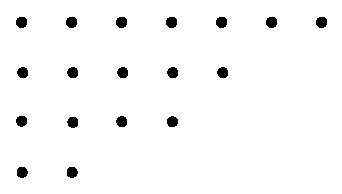
\includegraphics{figure/fig2.1.eps}
\caption{}\label{fig2.1}
\end{figure}

We will use summation convention here afterwards. Let 
\begin{align}\label{chap2:eq2.21}
a(u, v) &= \int\limits_\Omega\left(a_{ij}(x)\frac{\partial u} {\partial
  x_i} \frac{\partial v}{\partial x_j}+a_\circ \; uv\right)\,dx,\\
L(v) &= \int\limits_\Omega fv \,dx +\int\limits_\Gamma
gv\,d\Gamma, \label{chap2:eq2.22} 
\end{align}
where $a_\circ >0, a_{ij}$ are smooth and there exists two constants
$\alpha_\circ$ and $\alpha_1$ such that 
\begin{equation}\label{chap2:eq2.23}
\alpha_1 \xi_i\xi_i\geq a_{ij}(x)\xi_i\xi_j\geq\alpha_\circ\xi_i\xi_i
\quad\text{for all} x\varepsilon\Omega, \xi \varepsilon \mathbb{R}^n
\end{equation}
i.e. the quadratic form $a_{ij}(x)\xi_i\xi_j$ is uniformly continuous
and uniformly positive definite.

Inequality \eqref{chap2:eq2.23} implies that the bilinear form
$a(\cdotp,\cdotp)$ is continuous and $V$-coercive. Formally we have 
\begin{equation}\label{chap2:eq2.24}
a(u, v)=\int\limits_\Omega\left[-\frac{\partial}{\partial x_j} \left(a_{ij}
  \frac{\partial u}{\partial x_i}\right)v+a_\circ uv\right]\,dx+
\int\limits_\Gamma a_{ij}\frac{\partial u}{\partial x_i}n_jv\,d\Gamma
\end{equation}\pageoriginale
Let
$$
\frac{\partial u}{\partial v_A}=a_{ij}\frac{\partial u}{\partial x_i}
n_j, 
$$
and
$$
Au= -\frac{\partial}{\partial x_j}\left(a_{ij} \frac{\partial u} {\partial
x_i}\right). 
$$
If $v\varepsilon\mathscr{D}(\Omega)$ then the equation
\begin{equation}\label{chap2:eq2.25}
a(u, v)=L(v)
\end{equation}
becomes
$$
\langle Au, v\rangle= \langle f, v\rangle.
$$
Therefore
\begin{equation}\label{chap2:eq2.26}
Au=f\quad\text{in}\quad\mathscr{D}'(\Omega).
\end{equation}

Now for all $v\varepsilon V$, we have 
\begin{align*}
a(u, v) &= \int\limits_\Omega Au.v+\int\limits_\Gamma \frac{\partial
u}{\partial v_A}v\; d\Gamma\\
&= \int\limits_\Omega Au.v+\int\limits_{\Gamma_1} \frac{\partial u}
{\partial v_A}v\; d\Gamma\\
L(v) &= \int\limits_\Omega fv\,dx +\int\limits_{\Gamma_1} gv\,d\Gamma. 
\end{align*}

Equations \eqref{chap2:eq2.25} and \eqref{chap2:eq2.26} imply, for all
$v\varepsilon V$, 
$$
\int\limits_{\Gamma_1}\frac{\partial u}{\partial v_A}v\, d\Gamma =
\int\limits_{\Gamma_1} g\; v\, d\Gamma.
$$
From this we obtain formally
\begin{equation}\label{chap2:eq2.27}
\frac{\partial u}{\partial v_A}=g\quad\text{on}\quad\Gamma_1.
\end{equation}

Thus\pageoriginale the boundary value problem corresponding to the
variational problem
$$
a(u, v)=L(v)\quad\text{for all } v\varepsilon V,
$$
with $a(\cdotp,\cdotp), L(\cdotp)$ and $V$ given by the equations
\eqref{chap2:eq2.20} - \eqref{chap2:eq2.22} is
\begin{equation}\label{chap2:eq2.28}
\begin{split}
Au &= f\quad\text{in}\quad\Omega,\\
\frac{\partial u}{\partial v_A} &= g\quad\text{on}\quad\Gamma_1,\\
u &= 0\quad\text{on}\quad\Gamma_\circ.
\end{split}
\end{equation}

\begin{REM}\label{chap2:rem3}
Even when $f$ and $g$ are smooth the solution $u$ of the problem
\eqref{chap2:eq2.28} may not be in $H^2(\Omega)$. In general, we will
have a singularity at the transition points $A, B$ on $\Gamma$. But if
$\Gamma_\circ$ and $\Gamma_1$ make a corner then the solution $u$ may
be in $H^2(\Omega)$ provided that the boundary functions $f, g$
satisfy some compatibility conditions. For regularity theorems the
reader is referred to an article by PIERRE GIRSVARD \cite{key22}.
\end{REM}

\setcounter{exer}{0}
\begin{exer}\label{chap2:exr1}
{\bf Transmission Problem.} Let $\Omega, \Omega_1, \Omega_2$ be open
sets such that $\Omega =\Omega_1\cup\Omega_2\cup S$ where $\Omega_1$
and $\Omega_2$ are disjoint subsets of $\Omega$ and $S$ is the
interface between them. Let 
\end{exer}
\begin{align*}
a(u, v) &= \sum\limits_{i=1}^2\int\limits_{\Omega_i}a_i\nabla
u.\nabla v\,dx,\\
L(v) &= \int\limits_\Omega fv\,dx, 
\end{align*}
where\pageoriginale $a_i>0, i=1, 2$, and $f\varepsilon
L^2(\Omega)$. If $u$ is the solution of the problem
$$
a(u, v)=L(v)\quad\text{for all } v\varepsilon H_\circ^1(\Omega),
$$
and
$$
u_i=u|_{\Omega_i}, f_i=f|_{\Omega_i}
$$
then show that 
\begin{align*}
-a_i\Delta u_i &= f_i\quad\text{on}\quad\Omega_i, i=1, 2;\\
u_1 &= u_2\quad\text{on}\quad S,\\
a_1\frac{\partial u_1}{\partial n} &= a_2\frac{\partial u_2} {\partial
  n}\quad\text{on}\quad S.
\end{align*}
\begin{figure}[H]
\centering
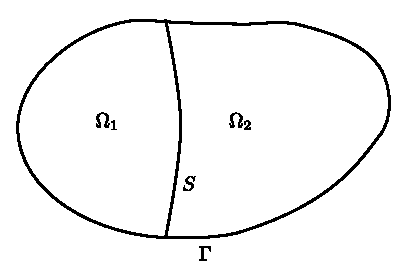
\includegraphics{figure/fig2.2.eps}
\caption{}\label{fig2.2}
\end{figure}

\begin{exer}\label{chap2:exr2}
{\bf Fourier Condition.} Let 
\begin{align*}
V &= H^1(\Omega),\\
a(u, v) &= \int\limits_\Omega\nabla u.\nabla v\,dx +
\int\limits_\Gamma uv\,d\Gamma,\\
L(v) &= \int\limits_\Omega fv\,dx + \int\limits_\Gamma gv\,d\Gamma,%%%%
\end{align*}
What is the boundary value problem associated with this \@? Interpret
the problem.
\end{exer}

\section{Elasticity Problem.}\label{chap2:ssec2.5}
\begin{itemize}
\item [(a)] {\bf 3-DIMENSIONAL CASE.}\pageoriginale Let $\Omega
  \subset \mathbb{R}^3$ be a bounded, connected open set. Let $\Gamma$
  be the boundary of $\Omega$ and let $\Gamma$ be split into two parts
  $\Gamma_\circ$ and $\Gamma_1$. Let $\Omega$ be occupied by an
  elastic medium, which we assume to be continuous. Let the elastic
  material be fixed along $\Gamma_\circ$. Let $(f_i)$ be the body
  force acting in $\Omega$ and $(g_i)$ be the pressure load acting
  along $\Gamma_1$. Let $(u_i(x))$ denote the displacement at $x$.
\begin{figure}[H]
\centering
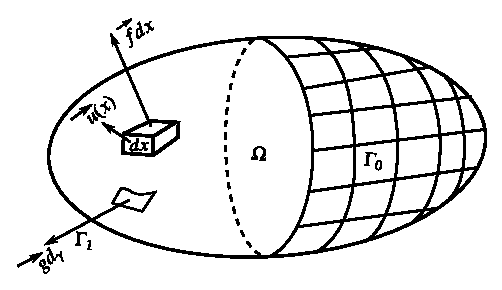
\includegraphics{figure/fig2.3.eps}
\caption{}\label{fig2.3}
\end{figure}


In linear elasticity the stress-strain relation is 
\begin{equation}\label{chap2:eq2.29}
\sigma_{ij.}(u)=\lambda(div \; u)\delta_{ij}+2\mu\varepsilon_{ij}(u),
\varepsilon_{ij}(u)=\frac{1}{2}\left(\frac{\partial u_i} {\partial
  x_j}+\frac{\partial u_j}{\partial x_i}\right),
\end{equation}
where $\sigma_{ij}$ and $\varepsilon_{ij}$ denote the components of the
stress and strain tensors respectively.


The problem is to find $\sigma_{ij}$ and $u_i$, given $(f_i)$ in
$\Omega$, $(g_i)$ on $\Gamma_1$ and $(u_i)=0$ on $\Gamma_\circ$.

The equations of equilibrium are
\begin{align}
\frac{\partial}{\partial
x_j}\sigma_{ij}+f_i &= 0\quad\text{in}\quad\Omega,\label{chap2:eq2.30}\\
\sigma_{ij}n_j &= g_i\quad\text{on}\quad\Gamma_1,\; i=1, 2, 3\tag{2.30b}\\
u_i &= 0\quad\text{on}\quad\Gamma_\circ.\tag{2.30c}
\end{align}\pageoriginale
We have used the summation convention in the above equations. We
choose
\begin{equation}\label{chap2:eq2.31}
v = \left\{v\varepsilon(H^1(\Omega))^3:v=0\quad\text{on}\quad\Gamma_\circ\right\},
\end{equation}
\begin{align}
a(u, v) &= \int\limits_\Omega\sigma_{ij}(u)\varepsilon_{ij}(v)\,dx, 
\label{chap2:eq2.32}\\
L(v) &= \int\limits_{\Gamma_1}g_iv_i\,d\Gamma +\int\limits_\Omega
f_iv_i\,dx.\label{chap2:eq2.33} 
\end{align}
Using \eqref{chap2:eq2.29}, $a(u, v)$ can be written as 
$$
a(u, v)=\int\limits_\Omega(\lambda \Div u.\Div v+2\mu\varepsilon_{ij}
(u)\varepsilon_{ij}(v))\,dx,
$$
from which it is clear that $a(\cdotp,\cdotp)$ is symmetric. That
$a(\cdotp,\cdotp)$ is $V$-elliptic is a nontrivial statement and the
reader can refer to CIARLET \cite{key9}. Formal application of Green's formula
will show that the boundary value problem corresponding to the
variational problem \eqref{chap2:eq2.31} - \eqref{chap2:eq2.33} is
\eqref{chap2:eq2.30}. 

$a(\cdotp,\cdotp)$ can be interpreted as the internal work and
$L(\cdotp)$ as the work of the external loads. Thus, the equation 
$$
a(u, v)=L(v)\quad\text{for all } v\varepsilon V
$$
is a reformulation of the theorem of virtual work.
\item [(b)] {\bf PLATE\pageoriginale PROBLEM.} Let $2\eta$ be the
  thickness of the plate. By allowing $\eta\to 0$ in (a) we obtain the
  equations for the plate problem. It will be a two dimensional
  problem.

We have to find the bending moments $M_{ij}$ and displacement
$(u_i)$. These two satisfy the equations:
\begin{equation}\label{chap2:eq2.34}
M_{ij}=\alpha\Delta u\delta_{ij}+\beta\frac{\partial^2u} {\partial x_i
\; \partial x_j},
\end{equation}
\begin{align}
\frac{\partial^2M_{ij}}{\partial x_i\;\partial x_j} &= f\quad\text{in}
\quad\Omega,\label{chap2:eq2.35}\\ 
u &= 0\quad\text{on}\quad\Gamma,\label{chap2:eq2.36}
\end{align}
and 

\begin{equation}\label{chap2:eq2.37}
\frac{\partial u}{\partial n}=0 \quad\text{if the plate is clamped},
\end{equation}
\begin{equation*}\label{chap2:eq2.37a}
M_{ij}n_in_j=0\quad\text{if the plate is simply supported}\tag{2.37a}
\end{equation*}
We take
\begin{equation}\label{chap2:eq2.38}
V=
\begin{cases}
H_\circ^2(\Omega)=\left\{ v\varepsilon H^2:V=\frac{\partial v} {\partial
n}=0 \quad\text{on}\quad\Gamma\right\},\\ 
\qquad\qquad\text{if the plate is clamped};\\
H^2(\Omega)\cap H_\circ^1(\Omega),\quad\text{if the plate is simply supported}
\end{cases}
\end{equation}
Formally, using Green's formula we obtain 
\begin{align*}
\int\limits_\Omega\frac{\partial^2M_{ij}}{\partial x_i\partial x_j}v\,
dx&= -\int\limits_\Omega\frac{\partial M_{ij}} {\partial x_j}
\frac{\partial v}{\partial x_i}\,dx+\int\limits_\Gamma \frac{\partial
  M_{ij}}{\partial x_j}vn_i\,d\Gamma\\
&=\int\limits_\Omega M_{ij}\frac{\partial^2v}{\partial x_i\partial x_j}\,
dx-\int\limits_\Gamma M_{ij}n_j\frac{\partial v}{\partial
  x_i}\,d\Gamma\\
&\qquad+\int\limits_\Gamma\frac{\partial M_{ij}}{\partial x_j}vn_i\,d\Gamma
\quad\text{for all } v\varepsilon V.\tag{2.39}\label{chap2:eq2.39}
\end{align*}
But\pageoriginale
$$
\int\limits_\Gamma\frac{\partial M_{ij}}{\partial x_j}vn_i\,d\Gamma =0
\quad\text{for all } v\varepsilon V,\quad\text{since}\quad v=0
\quad\text{on}\quad\Gamma,
$$
and
$$
\int\limits_\Gamma M_{ij}n_j\frac{\partial v}{\partial x_i}\,d\Gamma=
\int\limits_\Gamma M_{ij}n_j\left(n_i\frac{\partial v}{\partial n}+s_i
\frac{\partial v}{\partial s}\right)\,d\Gamma,
$$
where $\partial v/\partial n$ denotes the normal derivative of $v$ and
$\partial v/\partial s$ denotes the tangential derivative. By
\eqref{chap2:eq2.37} and \eqref{chap2:eq2.37a} we have 
$$
\int\limits_\Gamma M_{ij}n_j\frac{\partial v}{\partial x_i}\,d\Gamma=0. 
$$
Hence
$$
\int\limits_\Omega fv\,dx=\int\limits_\Omega \frac{\partial^2M_{ij}}
{\partial x_i\partial x_j}v\,dx=\int\limits_\Omega M_{ij}
\frac{\partial^2v}{\partial x_i\partial x_j}\,dx\quad\text{for all }
 v\varepsilon V.
$$
We therefore choose
\begin{equation}\label{chap2:eq2.40}
a(u, v)=\int\limits_\Omega M_{ij}\frac{\partial^2v}{\partial x_i
\partial x_j}\,dx=\int\limits_\Omega\left(\alpha\Delta u.\Delta v+\beta
\frac{\partial^2u}{\partial x_i\partial x_j}\frac{\partial^2v}
{\partial x_i\partial x_j}\right)\,dx
\end{equation}
and
\begin{equation}\label{chap2:eq2.41}
L(v)=\int\limits_\Omega fv\,dx.
\end{equation}

$a(\cdotp,\cdotp)$ can be proved to be $V$-coercive if $\beta\geq 0$
and $\alpha\geq 0$.
\end{itemize}

\setcounter{regthm}{3}
\begin{regthm}\label{chap2:rgthm4}
When $\Omega$ is smooth and $f\varepsilon L_2(\Omega)$, then the
solution $u$ of the problem 
\begin{align*}
-\Delta u &= f\quad\text{in}\quad\Omega,\\
u &= 0\quad\text{on}\quad\Gamma,
\end{align*}
belongs\pageoriginale to $H^2(\Omega)$. Moreover, we have 
$$
\parallel u\parallel_2\leq C\parallel f\parallel_\circ =C\parallel
\Delta u\parallel_\circ,
$$
where $C$ is a constant.
\end{regthm}

This proves the coerciveness of $a(u, v)$ above for $\beta =0$ and
$\alpha >0$. 

\section{Stokes Problem.}\label{chap2:ssec2.6}
The motion of an incompressible, viscous fluid in a region $\Omega$ is
governed by the equations
\begin{align}
-\Delta u+\nabla p &= f\quad\text{in}\quad\Omega,\label{chap2:eq2.42}\\
\Div u &= 0\quad\text{in}\quad\Omega,\label{chap2:eq2.43}\\ 
u &= 0\quad\text{in}\quad\Gamma;\label{chap2:eq2.44}
\end{align}
where $u=(u_i)_{i=1,\ldots,n}$ denotes the velocity of the fluid and
$p$ denotes the pressure. We have to solve for $u$ and $p$, given $f$.

We impose the condition \eqref{chap2:eq2.43} in the space $V$
itself. That is, we define
\begin{equation}\label{chap2:eq2.45}
V=\{v\varepsilon(H_\circ^1(\Omega))^n:\Div v=0\}
\end{equation}
Taking the scalar product on both sides of equation
\eqref{chap2:eq2.42} with $v\varepsilon V$ and integrating, we obtain 
$$
\int\limits_\Omega f.v\,dx=\int\limits_\Omega\frac{\partial u_i}
{\partial x_j}\frac{\partial v_i}{\partial x_j},
$$
since
\begin{align*}
-\int\limits_\Omega v.\Delta u &= -\int\limits_\Omega v_j
\frac{\partial^2u_j}{\partial x_i\partial x_i}\\
&= \int\limits_\Omega\frac{\partial v_j}{\partial x_i}.\frac{\partial
u_j}{\partial x_i}-\int\limits_\Gamma v_j\frac{\partial u_j} {\partial
x_i}n_i,
\end{align*}
and\pageoriginale 
$$
\int\limits_\Omega\nabla p.v=\int\limits_\Omega\frac{\partial p}
{\partial x_i}v_i=-\int\limits_\Omega p\frac{\partial v_i}{\partial
x_i}+\int\limits_\Gamma pv_in_i=0
$$
as $v\varepsilon V$. Therefore we define
\begin{align}
a(u, v) &= \int\limits_\Omega\frac{\partial u_i}{\partial x_j}
\frac{\partial v_i}{\partial x_j}\,dx \label{chap2:eq2.46}\\
L(v) &= \int\limits_\Omega f.v\,dx.\label{chap2:eq2.47}
\end{align}
We now have the technical lemma.
\setcounter{lem}{4}
\begin{lem}\label{chap2:lem5}
The space
$$
\vartheta=\left\{v\varepsilon(\mathscr{D}(\Omega))^n:\Div v=0\right\}
$$
is dense in $V$.
\end{lem}
The proof of this Lemma can be found in LADYZHENSKAYA \cite{key27}.

The equation $a(u, v)=L(v)$ for all $v\varepsilon V$ with $a(,),
L(\;), v$ defined by \eqref{chap2:eq2.45} - \eqref{chap2:eq2.47} is
then equivalent to 
\begin{equation*}\label{chap2:eq2.48}
\langle\Delta u+f, \phi \rangle=0\quad\text{for all }\phi\varepsilon\vartheta,
\tag{2.47} 
\end{equation*}
where $\langle , \rangle$ denotes the duality bracket between $(\mathscr{D}'
(\Omega))^n$ and $(\mathscr{D}(\Omega))^n$. Notice that
\eqref{chap2:eq2.47} is not valid for all $\phi\varepsilon
(\mathscr{D}(\Omega))^n$ since $(\mathscr{D}(\Omega))^n$ is not
contained in $\vartheta$. To prove conversely that the solution of
\eqref{chap2:eq2.47} satisfies \eqref{chap2:eq2.42}, we need

\setcounter{THM}{5}
\begin{THM}\label{chap2:THM6}
The annihilator $\vartheta^\bot$ of $\vartheta$ in
$(\mathscr{D}'(\Omega))^n$ is given by $\vartheta^\bot=\{v:$ there
exists a $p\varepsilon\mathscr{D}'(\Omega)$ such that $v=\nabla p\}$. 
\end{THM}

Theorem\pageoriginale \ref{chap2:ssec2.6} and Equation
\eqref{chap2:eq2.47} imply that there exists a $p\varepsilon
\mathscr{D}'(\Omega)$ such that 
$$
\Delta u+f=\Delta p.
$$

Since 
$$
u\varepsilon(H^1(\Omega))^n\quad\text{and}\quad f\varepsilon(L^2
(\Omega))^n, \Delta u+f\varepsilon(H^{-1}(\Omega))^n.
$$
Therefore
$$
\nabla p\varepsilon(H^{-1}(\Omega))^n.
$$

We now state

\begin{THM}\label{chap2:THM7}
If $p\varepsilon\mathscr{D}'(\Omega)$ and $\nabla p\varepsilon (H^{-1}
(\Omega))^n$, then $p\varepsilon L^2(\Omega)$ and 
$$
\parallel p\parallel_{L^2(\Omega)/\mathbb{R}}\leq C\parallel\nabla p
\parallel_{(H^{-1}(\Omega))^n}
$$
where $C$ is a constant.
\end{THM}

From this Theorem we obtain that $p \varepsilon L^2(\Omega)$. Thus, if
$f\varepsilon L^2(\Omega)$ and $\Omega$ is smooth, we have proved that
the problem \eqref{chap2:eq2.45} - \eqref{chap2:eq2.47} has a solution
$u\varepsilon V$ and $p\varepsilon L^2(\Omega)$. 
